\section{Experiments}\label{sec:experiments}
In this section, we detail the experiments conducted to evaluate the performance of each component within the MOC pipeline.
Our initial step was to establish a baseline using the replica of the MOC pipeline described in Section~\ref{sec:methodology}.
This baseline serves as a reference point for comparison and assessment of experimental results.

The experiments that follow are structured as follows:

\begin{enumerate}
    \item Evaluating the necessity of automated outlier removal in the PLS1-SM component by comparing performance with and without this process.
    \item Investigating the effect of fixed threshold values in the outlier removal process of PLS1-SM, maintaining these thresholds from the second iteration onwards.
    \item Assessing the impact of the Median Absolute Deviation (MAD) method for outlier removal in the Independent Component Analysis (ICA) phase.
    \item Determining the effect on ICA performance when utilizing datasets from five locations compared to a single dataset.
    \item Comparing the performance of PLS1-SM and ICA models against alternative models, such as XGBoost and Artificial Neural Networks (ANN).
\end{enumerate}

These experiments were selected to explore the significance of the outlier removal process, the optimization of threshold values, and the comparative effectiveness of different modeling approaches within the MOC pipeline.
The first experiment focuses on the automated outlier removal process in PLS1-SM, examining its necessity by comparing outcomes with and without this step.
The second experiment looks at the implications of using fixed threshold values for outlier removal in PLS1-SM, opting for a conservative approach by not updating these values after each iteration.
In the third experiment, we apply the MAD method for outlier removal in ICA, comparing its effectiveness against the baseline.
The fourth experiment evaluates ICA's performance using aggregated datasets from multiple locations, aiming to understand the balance between representativeness and information loss.
The final experiment extends the analysis to include comparisons with other models, providing a broader perspective on the MOC pipeline's performance.

This experimental approach allows for assessment of the MOC pipeline's components, offering insights into their individual and collective impacts on the system's overall performance.

\subsection{Replication of the MOC Pipeline}\label{sec:replica_moc}
We present the baseline RMSEs of the original and our replicas of the PLS1-SM, ICA, and MOC models in Table~\ref{tab:results_rmses}.
Figure~\ref{fig:rmse_histograms} illustrates the distribution of the RMSEs of the original and our replicas of the PLS1-SM, ICA, and MOC models as a grouped histogram.
The results show that the RMSEs of our replicas of the PLS1-SM, ICA and MOC models are similar to the original models.
However, the are some notable differences --- in some cases, our replicas outperform the original models, while in other cases, the original models outperform our replicas.
These differences can be attributed to a number of factors.

Firstly, the original models were trained on two datasets, one acquired at a 1600mm standoff distance and one acquired at a 3000mm standoff distance.
We have only used the 1600mm dataset for our replicas since we do not have access to the 3000mm dataset.
As mentioned in Section~\ref{sec:outlier_removal}, we also chose chose to automate the outlier removal process for the PLS1-SM phase, whereas the original authors performed this manually.
Moreover, we chose to exclude the outlier removal step during the ICA phase to avoid introducing unsubstantiated assumptions, as described in Section~\ref{sec:ica_data_preprocessing}.
In Section~\ref{sec:ica_data_preprocessing}, we clarified that unlike the original authors who utilized all five location datasets, our analysis was limited to a single dataset per sample due to the absence of details on their integration.
For training the PLS models, \citet{andersonImprovedAccuracyQuantitative2017} methodically organized their training and test sets by sorting samples based on the major oxide, sequentially assigning them to folds, removing outliers, and deliberately including extreme compositions in the training folds to enhance the model's ability to handle a broad range of elemental variations.
Since we lack the domain expertise to replicate this process, we instead randomly split the dataset into training and test sets without any further curation using a 80/20 split.
Additionally, without going into speculations, it is possible that some of the differences are due to implementation details, such as the use of different programming languages and libraries.
Lastly, it is worth noting that RMSE is simply a statistical measure of the differences between the original and predicted values, and does not necessarily reflect the true accuracy of the models on unseen data from Mars, and so the results should be interpreted with this in mind.

\begin{table*}[h]
\centering
\begin{tabular*}{\textwidth}{@{\extracolsep{\fill}}lllllll}
\hline
Element    & PLS1-SM (original) & PLS1-SM (replica) & ICA (original) & ICA (replica) & MOC (original) & MOC (replica) \\
\hline
\ce{SiO2}  & 4.33               & 5.81              & 8.31           & 10.68         & 5.30           & 7.29 \\
\ce{TiO2}  & 0.94               & 0.47              & 1.44           & 0.63          & 1.03           & 0.49 \\
\ce{Al2O3} & 2.85               & 1.94              & 4.77           & 5.55          & 3.47           & 2.39 \\
\ce{FeO_T} & 2.01               & 4.35              & 5.17           & 8.30          & 2.31           & 5.21 \\
\ce{MgO}   & 1.06               & 1.17              & 4.08           & 2.90          & 2.21           & 1.67 \\
\ce{CaO}   & 2.65               & 1.43              & 3.07           & 3.52          & 2.72           & 1.81 \\
\ce{Na2O}  & 0.62               & 0.66              & 2.29           & 1.72          & 0.62           & 1.10 \\
\ce{K2O}   & 0.72               & 0.72              & 0.98           & 1.37          & 0.82           & 1.09 \\
\hline
\end{tabular*}
\caption{RMSE of the original and our replicas of the PLS1-SM, ICA, and MOC models.}
\label{tab:results_rmses}
\end{table*}

\begin{figure*}[b]
	\centering
	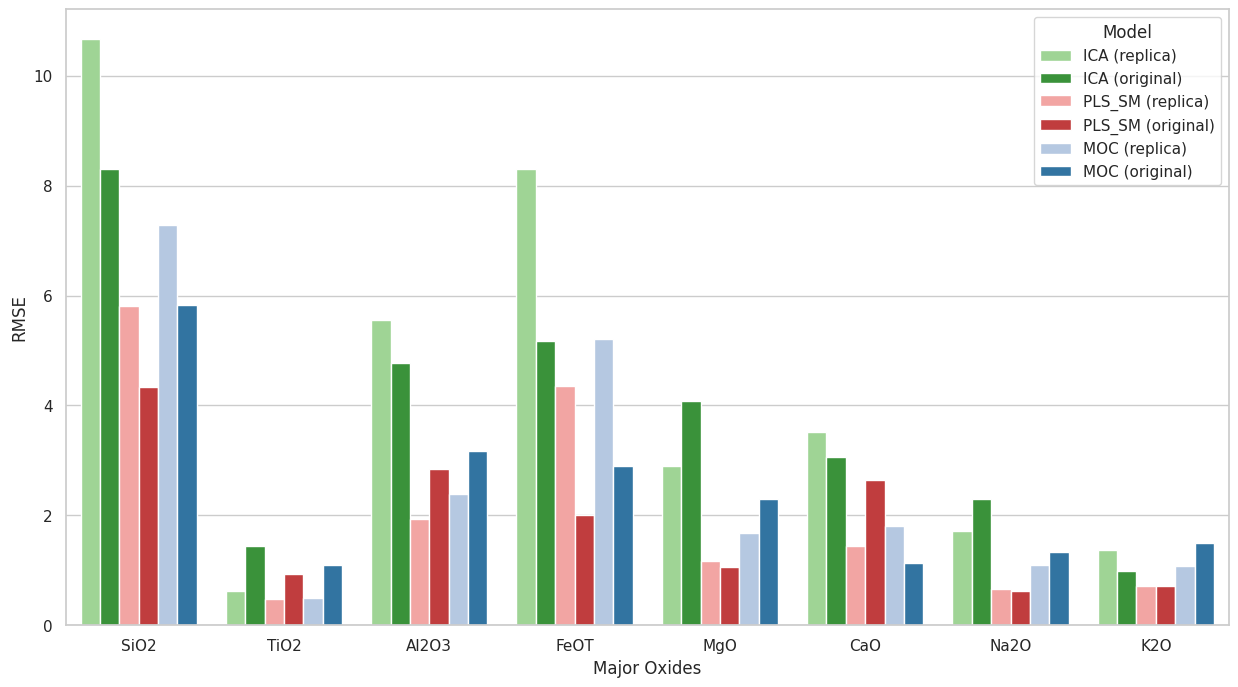
\includegraphics[width=0.85\textwidth]{images/rmse_historgram.png}
	\caption{Grouped histogram of the RMSEs of the original and our replicas of the PLS1-SM, ICA, and MOC models.}
	\label{fig:rmse_histograms}
\end{figure*}

\citet{andersonImprovedAccuracyQuantitative2017} used the Student's t-test to show their new model outperformed the old one. In our study, we apply the same test but with a different aim: to verify if there is no statistical significant difference between our replicated models (PLS1-SM, ICA, and MOC) and the original models presented in \citet{cleggRecalibrationMarsScience2017}. This approach allows us to assess whether our models demonstrate equivalence rather than improvement.
In conducting our analysis with the Student's t-test, we define our hypotheses and choose a significance level to guide our interpretation of the results.
Our null hypothesis (\(H_0\)) posits that there is no significant difference between the mean performance of our replicated models (PLS1-SM, ICA, and MOC) and that of the originals.
Conversely, the alternative hypothesis (\(H_1\)) suggests that there is a significant difference between the two sets of models.
We set a significance level (\(\alpha\)) of 5\%, which establishes the threshold for determining statistical significance.
If the p-value obtained from our t-test is less than 5\% (\(p < 0.05\)), we will reject the null hypothesis, indicating significant evidence of a difference between our replicated models and those of the original pipeline.
Conversely, if the p-value is greater than or equal to 5\% (\(p \geq 0.05\)), we fail to reject the null hypothesis, suggesting that our models and the original models are statistically similar, thereby achieving our goal of demonstrating equivalence rather than disparity.

Following the approach delineated in \citet{andersonImprovedAccuracyQuantitative2017}, we start by calculating the uncertainty of the RMSE values, $S_{RMSE}^2$:
$$
S_{\text{RMSE}}^2 = \left(\frac{\text{RMSE}^2}{n}\right) \left[n - 1 - \frac{2\Gamma^2\left(\frac{n}{2}\right)}{\Gamma^2\left(\frac{n - 1}{2}\right)}\right] \\
$$
where $n$ is the number of samples, and $\Gamma$ is the gamma function. This formulation captures the variance of the RMSE, reflecting the dispersion of error magnitudes.
Subsequently, the t-statistic $t$ is calculated to evaluate the statistical significance of the difference between the RMSEs of the original and replicated models:
$$
t = \frac{\text{RMSE}_A - \text{RMSE}_B}{\sqrt{S_{\text{RMSE}_A}^2 + S_{\text{RMSE}_B}^2}}
$$
where $\text{RMSE}_A$ and $\text{RMSE}_B$ correspond to the RMSE values of the original and replicated models, respectively.
The degrees of freedom ($f$) associated with this comparison are determined by:
$$
f = \frac{\left(S_{\text{RMSE}_A}^2 + S_{\text{RMSE}_B}^2\right)^2}{\frac{S^4_{\text{RMSE}_A}}{n_A - 1} + \frac{S^4_{\text{RMSE}_B}}{n_B - 1}}
$$
which accounts for the variances in RMSE values and the respective sample sizes ($n_A$ and $n_B$) of the models being compared.
Finally, the p-value is derived from the t-distribution's cumulative distribution function:
$$p\text{-value} = 2 \times \left(1 - F_{\text{T}}(|t|)\right)$$
where $F_{\text{T}}$ is the cumulative distribution function of the t-distribution with $f$ degrees of freedom. 
Higher p-values indicate greater compatibility with the null hypothesis.

We present the results of our t-tests in Table~\ref{table:results_ttests}.

\begin{table}[h]
\centering
\begin{tabular}{llll}
\hline
\textbf{Oxide} & \textbf{PLS1-SM} & \textbf{ICA} & \textbf{MOC} \\
\hline
\ce{SiO2} & 42.00\% & 48.75\% & 38.45\% \\
\ce{TiO2} & 9.73\% & 6.31\% & 8.23\% \\
\ce{Al2O3} & 30.23\% & 67.06\% & 31.58\% \\
\ce{FeO_T} & 7.48\% & 21.68\% & 6.57\% \\
\ce{MgO} & 78.05\% & 35.44\% & 44.08\% \\
\ce{CaO} & 12.73\% & 70.04\% & 27.79\% \\
\ce{Na2O} & 85.96\% & 43.16\% & 14.93\% \\
\ce{K2O} & 100.00\% & 36.27\% & 43.40\% \\
\hline
\end{tabular}
\caption{Results of the PLS1-SM, ICA, and MOC t-tests}
\label{table:results_ttests}
\end{table}

The results from our t-tests are summarized as follows:

\begin{itemize}
    \item \textbf{PLS1-SM:} The p-values observed across the spectrum, most notably the 100.00\% for $K_2O$, unequivocally suggest a strong statistical proximity to the original models for a majority of the parameters. This is particularly indicative of a successful replication effort. However, the relatively lower p-value for $FeO_T$ (7.48\%) underscores an area where the model's performance diverges from the original. Given the high variance noted in the Section~\ref{sec:data_overview} for $FeO_T$ compositions, this deviation could be ascribed to inherent data variability rather than model inaccuracy.

    \item \textbf{ICA:} This model demonstrates considerable alignment with the original models across several constituents, as evidenced by p-values like 67.06\% for $Al_2O_3$ and 70.04\% for $CaO$. These figures indicate a noteworthy approximation to the original models' performance. Conversely, the p-value for $TiO_2$ (6.31\%) marks an exception, indicating a region where the ICA model might benefit from refinement. The noted high variance in $TiO_2$ values within our dataset likely contributes to this outlier, pointing to data variability as a contributing factor.

    \item \textbf{MOC:} The replicated MOC model's p-values, especially the 43.40\% for $K_2O$, reiterate its consistency with the original model's outcomes. This aligns with our hypothesis of statistical equivalence. Yet, as with PLS1-SM, the $FeO_T$ component exhibits a lower p-value (6.57\%), highlighting an area of divergence potentially attributed to the previously discussed variance in $FeO_T$ compositions.
\end{itemize}

Our comparative analysis, enriched by an acknowledgment that higher p-values denote model fidelity, predominantly affirms the statistical equivalence of our replicated models to the original MOC models across most tested parameters.
This alignment underscores the robustness of our replication efforts.

However, the lower p-values associated with $FeO_T$ for both PLS1-SM and MOC, in addition to $TiO_2$ for ICA, flag these elements as focal points for potential refinement.
Given our dataset's inherent variability in the compositions of these specific elements, as substantiated in Section~\ref{sec:data_overview}, these findings are interpretable and not wholly unexpected.

In conclusion, our t-tests demonstrate that our replicated models are statistically similar to the original models, thereby achieving our goal of demonstrating equivalence rather than disparity.
As such, they serve their purpose as a baseline for identifying which aspects of the pipeline contribute the most to the overall error. 


\subsection{Experiment: Outlier Removal}\label{sec:experiment_outlier_removal}
% TODO: Add results and discussion.

The original PLS1-SM identified outliers manually by inspecting the leverage and spectral residuals plots.
We have instead chosen to automate this based on the reasons described in Section~\ref{sec:methodology_outlier_removal}.
It would therefore be intriguing to examine the impact on the pipeline's performance when this process is adjusted.
Firstly, examining the performance implications of completely omitting outlier removal would be worthwhile.
This experiment is justified given the substantial efforts dedicated to developing the ChemCam calibration dataset as mentioned in Section~\ref{sec:ica_data_preprocessing}, which implies a minimal presence of significant outliers.
Secondly, maintaining the threshold values from the second iteration of the outlier removal in the PLS1-SM training process would lead to a more conservative outlier removal process where fewer samples are removed.
The reason for doing so is that we do not know the basis for the original author's manual outlier removal process, and it is possible that they were more conservative than our automated process.
Consequently, a more conservative approach could potentially align our replica of the pipeline more closely with the original.

In the ICA phase, the original authors employed the Median Absolute Deviation (MAD) for outlier removal, yet the detailed methodology of their approach was not fully delineated.
Consequently, in our version of the pipeline, we chose to exclude the outlier removal step during the ICA phase to avoid introducing unsubstantiated assumptions, as described in Section~\ref{sec:ica_data_preprocessing}.
This decision allows us to evaluate the intrinsic effectiveness of the ICA phase without the influence of outlier removal.
Introducing outlier removal using MAD in our replication of the pipeline presents an opportunity to assess its impact on the pipeline's efficacy.
By comparing the results with and without MAD, we can quantitatively measure the utility of this step.
Such an experiment is crucial for understanding whether MAD significantly contributes to reducing noise and improving data quality, thereby enhancing the overall performance of the machine learning pipeline.
This experiment would also offer insights into the robustness of the ICA phase against outliers, providing a more comprehensive understanding of the pipeline's capabilities and limitations.

\subsection{Experiment: Other Models}\label{sec:experiment_other_models}
\citet{cleggRecalibrationMarsScience2017} have only compared their new approach with the original method presented by \citet{wiensPreFlight3}, and have not conducted experiments using alternative methods to establish the superiority of their chosen approach.
Therefore, we decided to compare the performance of the PLS1-SM and ICA models to other models.
The objective is to evaluate two distinct scenarios.
In the first scenario, we aim to conduct a direct comparison between the MOC model and an alternative model. The second scenario revolves around substituting either PLS or ICA with a different model and then calculating a weighted average.
We have decided to conduct the experiments using the following models:

\begin{itemize}
	\item \textbf{XGBoost}, a gradient boosting algorithm, \cite{chen_xgboost_2016}.
	\item \textbf{ANN}, a neural network model, \cite{scikit-learn}.
\end{itemize}

% TODO: Argue why we chose these models (ref SuperCam paper).
% TODO: Add results and discussion.